\documentclass[nogrid]{MBE}%


\usepackage{url}
\usepackage{nicefrac}
\usepackage[flushleft]{threeparttable}
\usepackage{adjustbox}

\jshort{mst}

\volname{}

\jvolume{0}

\jvol{}

\jissue{0}

\pubyear{2016}

\mstype{Article}

% \artid{012}

% \access{Advance Access publication March 3, 2013}


\begin{document}

\title[StarBEAST2]{StarBEAST2 brings faster species tree inference and accurate estimates of substitution rates}


\author[Ogilvie and Drummond]{Huw A. \surname{Ogilvie}$^{\ast,1,2}$ and Alexei J. Drummond$^{2,3}$}

\address{$^{1}$Division of Evolution, Ecology and Genetics, Research School of Biology, Australian National University, Canberra, Australia\\
$^{2}$Centre for Computational Evolution, University of Auckland, Auckland, New Zealand\\
$^{3}$Department of Computer Science, University of Auckland, Auckland, New Zealand}


% \history{Received 13 July 2011; reviews returned 26 November 2012; accepted 30 November 2012}

\coresp{E-mail: huw.ogilvie@anu.edu.au.}

% \editor{Robb Brumfield}

\abstract{Concatenation of multiple loci to infer a single tree is a popular
estimator of species tree topology and times, but is statistically inconsistent inside the
anomaly zone of short branch lengths. The ages of extant species inferred using
concatenation can also be severely overestimated. These known biases have
motivated the development and use of multispecies coalescent (MSC) methods of
species tree inference. Summary MSC methods like ASTRAL are becoming increasing
popular as they are fast enough to use with large phylogenomic data sets, but
cannot estimate divergence times and extract less information per gene compared
to fully Bayesian MSC methods like *BEAST. The continued focus on developing
summary methods which can only infer the topology of a species tree is
questionable, since the accuracy of concatenation when inferring branch lengths
is quantitatively worse than for topology. Instead of another summary method we
have developed StarBEAST2, a fully Bayesian MSC method with improved
computational performance. StarBEAST2 will enable inference of more accurate
species trees and divergence times by increasing the maximum number of loci that
is practical for a given analysis. StarBEAST2 also adds support for species tree
relaxed clocks, and we show that unlike concatenation it can accurately estimate
per-species substitution rates. StarBEAST2 is available through the BEAUTi
package manager in BEAST 2.4 and above.}

\keyword{Phylogenetic methods, substitution rate, relaxed clock, multispecies coalescent, concatenation.}

\maketitle

\section{Introduction}

The throughput of sequencing technologies has improved many-fold over the past
two decades, culminating in next generation sequencing (NGS), and it is now
feasible to sequence whole or partial genomes or transcriptomes for phylogenetic
studies \citep{annurev-ecolsys-110512-135822}. NGS produces hundreds or
thousands of phylogenetically useful loci \citep[see for example][]{Blom056085},
with potentially millions of sites spread across a data set of multiple
sequence alignments.

\newpage

While NGS offers hundreds or thousands of loci at relatively low cost, making
accurate inferences from the enormous amount of data produced is particularly
challenging. In the case of *BEAST, a fully Bayesian method of species tree
inference which implements a realistic and robust evolutionary model in the
multispecies coalescent \citep[MSC;][]{Degnan2009332, Heled01032010}, it becomes exponentially
slower as the number of loci in an analysis is increased. This scaling behaviour
causes *BEAST to become intractably slow after a certain number of loci
\citep[the exact number will depend on the other parameters of the data set, see][]{Ogilvie01052016}.
Given the current challenges of using large phylogenomic data sets with *BEAST
there have been three broad alternatives available to researchers; concatenate
sequences from multiple loci, use alternative MSC methods which are based on
summary statistics instead of the full sequence data, or choose a tractable
subset of loci to use with *BEAST.

Concatenating sequences from multiple loci will reconstruct the single tree that
best fits the combined sequence alignment. Popular concatenation methods include
the RAxML and ExaML maximum likelihood methods \citep{Stamatakis01052014,
Kozlov01082015}, and the ExaBayes and BEAST Bayesian methods
\citep{Aberer01102014, Drummond2007}. Recent results show that concatenation
can be counterproductive, producing statistically inconsistent results which assign
high confidence to incorrect nodes due to model misspecification
\citep{NYAS:NYAS12747}. In the so-called ``anomaly zone'' of short branch
lengths, the most likely gene tree topology will be different from the species
tree, and concatenated tree topologies will likely differ from the true species
tree topologies \citep{journal.pgen.0020068, Kubatko01022007}.

More recently identified problems with concatenation are overestimation of
divergence times and systematic error when estimating substitution rates. Branch lengths
inferred by concatenation will reflect the expected number of substitutions per
site across all concatenated loci. Divergence times, as determined by branch
lengths on a time tree, will therefore reflect the average coalescence times of
all genes. This misspecification leads to overestimation which can be
particularly severe in terms of the ages of extant species
\citep{Ogilvie01052016}. Trees inferred using concatenation are therefore not a
reliable approximation of the species tree in terms of branch lengths or
topology. Per-species substitution rates inferred using a relaxed clock model
with concatenation may also be substantially overestimated or underestimated
depending on their relationship with the gene trees \citep{Mendes28022016}.

As an alternative to concatenation, MSC methods which use summary statistics instead
of the full sequence data have been developed for use with phylogenomic data.
Popular summary methods include MP-EST and ASTRAL \citep{Liu2010,
Mirarab01092014}, but recent results show that MP-EST should be avoided as it is
sensitive to gene tree error \citep{Mirarab15062015, Xi201563}. At low levels of
incomplete lineage sorting (ILS) MP-EST is less accurate than concatenation at
inferring topologies, and even at high levels of ILS it may be no more accurate
than concatenation \citep{Ogilvie01052016}. While other summary methods like
ASTRAL may be more reliable than MP-EST, none of these methods can infer branch
lengths in substitution units. Divergence times therefore cannot be
reconstructed using summary methods. If concatenation is used to estimate branch
lengths, divergence times, and/or substitution rates for a fixed species tree
topology estimated using a summary method, then those estimates will be
unreliable for the same reasons as pure concatenation.

With the aim of improving the computational performance of fully Bayesian
MSC inference of species trees we have developed an upgrade
to *BEAST called ``StarBEAST2'', which is available as a package for BEAST 2
\citep{10.1371/journal.pcbi.1003537}. By improving computational performance
StarBEAST2 should enable the use of more loci, thereby improving the precision
of estimated parameters and providing an alternative to concatenation. We have
also developed and include in StarBEAST2 a new MSC relaxed
clock model to enable accurate inference of per-species substitution rates.

\section{New Approaches}

\subsection{Analytical integration of population sizes}

Markov Chain Monte Carlo (MCMC) methods like *BEAST simultaneously integrate
over many parameters by proposing small changes at each step to eventually
produce a probability distribution for all parameters. From a
researcher's perspective, some may be ``nuisance'' parameters not of scientific
interest. For example species tree topology and divergence times may be of
interest, but not effective population sizes. For tractable parameters, an
analytic solution will integrate over the entire range of values at each MCMC
step, and may be more high performance than MCMC integration. However explicit
estimates will not be produced so this approach is suitable only for nuisance
parameters. Among-site rate variation is already integrated out at each step;
the likelihood of each site is calculated for all possible discrete gamma rates
at each step, so the individual site rates are not estimated \citep{Yang1994}.

Analytical integration of constant per-branch population sizes was first
implemented as part of BEST \citep{EVO:EVO414}. The analytic solution, which
we have added to StarBEAST2, uses an inverse gamma conjugate prior for
population sizes. By default StarBEAST2 fixes the shape of the distribution
$\alpha = 2$ and only estimates the scale $\beta$. Because the mean of an
inverse gamma distribution is equal to $\nicefrac{\beta}{\alpha - 1}$, under default
settings the hyperparameter $\beta$ is an estimate of mean effective
population size.

\subsection{Coordinated tree topology changing operators}

One approach to improving the performance of MSC analyses which simultaneously
estimate gene and species trees (such as *BEAST) is to develop MCMC operators
which propose coordinated changes to both the species tree and the gene trees in
the same step. \cite{Yang01122014} and \cite{2015arXiv151203843R} introduced
Metropolis-Hastings (MH) operators which make nearest-neighbor interchange (NNI) and subtree prune and regraft (SPR) changes to the species
tree topology, and simultaneously make changes to the gene tree topologies that
preserve compatibility of the gene trees within the proposed species tree. We have
reimplemented those operators as a new operator in StarBEAST2 called
``CoordinatedExchange''. \cite{2015arXiv151203843R} also describe a proposal
distribution which favours topological changes on shorter branches, and also
less radical changes in topology. StarBEAST2 implements a simpler proposal
distribution but still favours less radical changes by applying adjustable
proposal probability weights to (less radical) NNI moves and (more radical) SPR
moves.

\subsection{Coordinated node height changing operators}

A novel class of coordinated Metropolis operators was introduced by
\cite{Jones010199}. These operators change the height of a non-root non-leaf
species tree node, and the heights of ``connected components'' of gene tree
nodes, by an amount $\epsilon$ chosen from a uniform distribution.
The lower bound of the uniform distribution is the negative length of
the shortest child branch of any connected component or of the species tree node,
and the upper bound is the positive length of the shortest parent branch. As
long as the connected components are chosen with reference only to the topology
of the species tree, the topology of the gene trees, and the mapping of
sampled individuals to species, operators of this class are symmetric
\citep{Jones010199}.

We have developed a new operator called ``CoordinatedUniform'' that belongs to
this class. Individuals from extant species which descend from a species tree
node, or are directly descended from a gene tree node, are referred to as
descendant individuals. The gene tree nodes selected by this operator are those
for which (1) at least one descendant individual is also a descendant individual
per direct child of the selected species tree node and (2) all descendent
individuals are also descendent individuals of the selected species tree node.

We have also developed a new adaptive MH \citep{Andrieu2008} operator called
``CoordinatedExponential'' which changes the height of the species tree root and
the height of connected components of gene tree nodes by an amount $\epsilon$.
The changed gene tree nodes are those for which at least one descendant individual
is also a descendant individual per direct child of the species tree root.
Because the length of parent branches of the species tree root or connected
components will be undefined, a different method must be used to choose
$\epsilon$ compared to CoordinatedUniform.

First the lower bound of the species tree root height is defined as the current
height minus the length of the shortest child branch of any connected component or
of the species tree root. The difference between the lower bound and the current
root height is referred to as $x$, and a new random value $x'$ is chosen from an
exponential distribution. The value of $x' - x$ is then used for $\epsilon$. The
median of the exponential distribution is adaptively modified over the course of
an MCMC chain to equal the posterior expectation of $x$.

Because the proposal distribution for a new species tree root height is
independent of the current height, the Hastings ratio which is usually
$\nicefrac{q(x',x)}{q(x,x')}$ \citep{Hastings1970} can be simplified to
$\nicefrac{\pi(x)}{\pi(x')}$. The natural logarithm of the Hastings ratio may then
be derived from the respective probability densities of $x$ and
$x'$ drawn from an exponential distribution with the rate $\lambda$:

\begin{align}
\frac{\pi(x)}{\pi(x')} &= \frac{\lambda e^{-\lambda x}}{\lambda e^{-\lambda x'}} = \frac{e^{-\lambda x}}{e^{-\lambda x'}}\\
\therefore \ln\left(\frac{\pi(x)}{\pi(x')}\right) &= \ln\left(e^{-\lambda x}\right) - \ln\left(e^{-\lambda x'}\right)\\
& = \lambda x' \cdot \ln\left(e\right) - \lambda x \cdot \ln\left(e\right)\\
& = \lambda \left(x' - x\right) = \lambda \epsilon
\end{align}

\subsection{Species tree relaxed clocks}

The overall rate of evolution occurring at a given locus within a species will
be influenced by the nature of the particular gene and also by the natural
history of the particular species. For a given gene, the average substitution
rate may depend on neutral processes such as the timing of replication for the
corresponding genomic region in humans \citep{Stamatoyannopoulos2009}, or the
effects of selection such as the faster molecular evolution of sex-biased genes
in \textit{Arabidopsis thaliana} \citep{Gossmann01032014}. For a given species,
the average substitution rate is correlated with a multitude of traits including
metabolic rate, body size, and fecundity, although causal relationships are
difficult to pin down \citep{Bromham2503}. Unsurprisingly, empirical analysis
has shown that two major factors contributing to rate variation among gene
branches is the per-gene rate and the per-species rate
\citep{Rasmussen01122007}.

Because variation is expected in the nature of different genes and species, and
therefore variation is also expected in the average substitution rate of different
genes and species, multispecies coalescent models should take both per-gene and
per-species rate variation into account. *BEAST can accommodate both types of
rate variation using gene tree relaxed clock models \citep[for examples see][]{Berv2014120, Lambert2015146}.
This involves estimating per-branch substitution rates (branch rates) separately
for each branch of each gene tree. While gene tree relaxed clocks may
accommodate variation in substitution rates between species, they do not produce
estimates of species branch rates. To enable accurate inference of species
branch rates, we have developed a new species tree relaxed clock model.

The challenge of applying a relaxed clock to the species tree is that
phylogenetic likelihood calculations require branch rates for each branch of
each gene tree. Our clock model uses the total expected number of substitutions
$\Sigma \mathbb{E}(S)$ accumulated by a gene branch through all containing
species branches. Substitutions are expected to be accumulated at the mean
clock rate of the gene tree $c$, for example 0.01 for hominoid primate
mitochondrial DNA \citep{doi:10.1146/annurev.es.18.110187.001413}, multiplied
by the lengths of time $L$ spent traversing each species tree branch, multiplied
by the rates $R$ of the corresponding species tree branches
(Table~\ref{tab:branchRateModel}).

\begin{table*}[htb!]
\caption{Expected numbers of substitutions $\Sigma \mathbb{E}(S)$ under a species tree relaxed clock}
\label{tab:branchRateModel}
\begin{threeparttable}
\begin{tabular*}{\textwidth}{@{\extracolsep{\fill}}cccccccccccc@{}}
\hline
Gene & Gene & \multicolumn{3}{c}{Length within $L$} & \multicolumn{3}{c}{Species rate $R$} & \multicolumn{3}{c}{$\mathbb{E}(S) = c\cdot L\cdot R$} & \multirow{2}{*}{$\Sigma \mathbb{E}(S)$}\tabularnewline
branch & rate $c$ & A & B & AB & A & B & AB & A & B & AB & \tabularnewline
\hline
a & \multirow{2}{*}{0.01} & 1.0 & 0.0 & 0.5 & \multirow{2}{*}{0.7} & \multirow{2}{*}{1.0} & \multirow{2}{*}{1.3} & 0.0070 & 0.0000 & 0.0065 & 0.0135\tabularnewline
b & & 0.0 & 1.0 & 0.5 & & & & 0.0000 & 0.0100 & 0.0065 & 0.0165\tabularnewline
\hline
\end{tabular*}
\end{threeparttable}
\end{table*}

The gene tree branch rates $r$ can then be derived by dividing the total
expected number of substitutions by the total length of that branch $l$. The
gene tree branch rates for the illustrated example
(Figure~\ref{fig:branchRateModel}; Table~\ref{tab:branchRateModel}) are
therefore:

\begin{align}
r_a &= \frac{\Sigma \mathbb{E}(S_a)}{l_a} = \frac{0.0135}{1.5} = 0.009\\
r_b &= \frac{\Sigma \mathbb{E}(S_b)}{l_b} = \frac{0.0165}{1.5} = 0.011
\end{align}

The new species tree relaxed clock model is available in StarBEAST2. Branch rate
models that can be used with a species tree relaxed clock currently include the
well-established uncorrelated log-normal (UCLN) and uncorrelated exponential
(UCED) models \citep{10.1371/journal.pbio.0040088}, as well as the newer random
local clock (RLC) model \citep{Drummond2010}.

\begin{figure}[htb!]
\centering
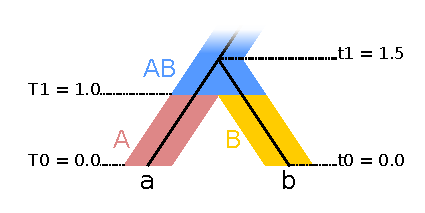
\includegraphics[width=8cm]{relaxed_clock.pdf}
\caption
{Multispecies coalescent phylogeny used to illustrate species tree relaxed
clocks. There are two extant species ``A'' and ``B'', and one ancestral species ``AB''.
Within the species tree there is a single gene tree with extant individuals ``a''
and ``b''. The single speciation event occurs at time T1, and the single coalescence
event occurs at time t1.}
\label{fig:branchRateModel}
\end{figure}

\section{Results}

\subsection{StarBEAST2 correctly implements the multispecies coalescent}

New methods must be shown to be mathematically correct implementations of the
target model. One way to accomplish this for MCMC methods is to estimate
parameters from a prior distribution using the MCMC kernel, and to also draw
independent samples from an identical distribution by simulation. The resulting
parameter distributions should be identical if the implementation is correct. We
used this method to test the correctness of the novel features in StarBEAST2;
analytical population size integration, coordinated operators, and species tree
relaxed clocks. Simulated and StarBEAST2 estimated distributions were identical
for species and gene tree topologies (Figure~S1,S2), species and gene tree node
heights (Figure~S3,S4), and for gene tree branch rates (Figure~S5,S6). This
combination of results supports the correctness of the StarBEAST2
implementation.

\subsection{\textit{Pseudacris} chorus frogs have intermediate coalescent branch lengths}

To characterize the performance of coordinated operators, methods of population size
integration and relaxed clocks, we tested StarBEAST2 using real sequence data.
The data set used for this analysis is from the North American chorus frog genus
\textit{Pseudacris}, and was originally collected and analyzed by
\cite{Barrow201478}. A key metric of phylogenies that can be used to judge
whether it is necessary to employ MSC models is the average
branch length in coalescent units $\nicefrac{\tau}{2Ne}$. Given short branch
lengths, concatenation is unable to infer accurate species trees regardless of
the number of loci used, but for long branch lengths, concatenation is
approximately as accurate as *BEAST \citep{Ogilvie01052016}. Using StarBEAST2,
the average branch length within this genus was determined to be
$\nicefrac{1.69\tau}{2Ne}$. This is an intermediate average length, longer than
the shallow simulations analyzed by \cite{Ogilvie01052016} which had a short
average length of $\nicefrac{0.54\tau}{2Ne}$.

\subsection{Coordinated height changing operators and analytical integration improve performance}

To determine which configuration of new features would achieve the best
performance, we ran StarBEAST2 using different combinations of operators,
methods of population size integration and different relaxed clocks. To measure
convergence both effective sample size (ESS) per hour and ESS per million states
were computed for each independent chain. ESS per hour can be used to calculate
the total time required for a converged chain (nominally where ESS equals or
exceeds 200), and reflects how effectively operators explore the space of trees
and parameters, and the computational time required by each operator proposal
and likelihood calculation. In contrast, ESS per million states reflects only
the exploration of tree and parameter space independently of calculation times.
A variety of statistics were logged for each analysis, but the height of the
species tree had the slowest average convergence rates so we used that statistic
to judge computational performance (Table~S1,S2).

Multiple linear regressions with log transformed ESS rates as the response
variables were used to measure the effect of adding topology changing operators,
node height changing operators, and of the method of population size
integration. Each additional feature was treated as a binary indicator variable, so that
we were able to quantify the change in performance as a percentage by
exponentiating the coefficient for each addition
(Table~\ref{tab:convergenceLM}).

Coordinated topology operators had a negative effect on ESS per hour of gene
tree relaxed clock analyses, regardless of the addition of height changing
operators or the method of population size integration
(Figure~\ref{fig:realEssPerHour}). There was no change to ESS per million states
(Figure~\ref{fig:realEssPerMstates}), and it made no significant difference to the
convergence of species tree relaxed clock analyses
(Table~\ref{tab:convergenceLM}). These results suggest that coordinated topology
operators are not substantially more effective than na\"ive operators at
proposing new states.

\begin{figure}[htb!]
\centering
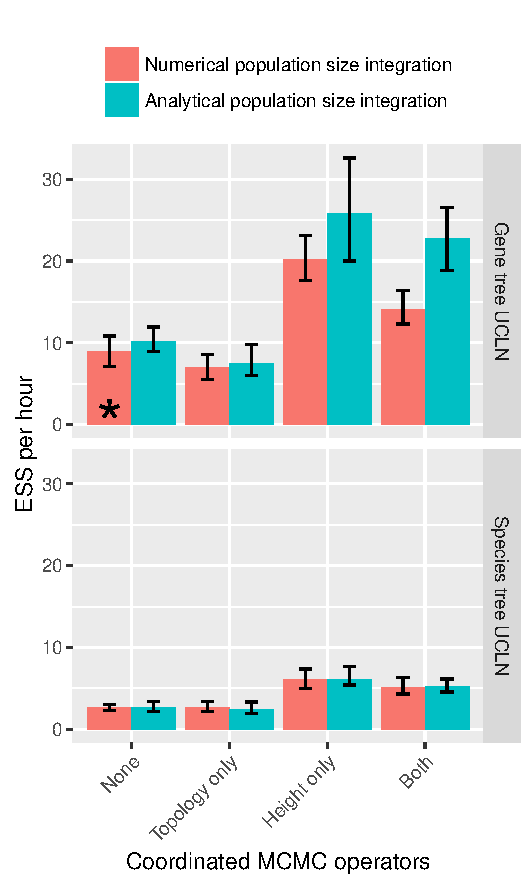
\includegraphics[width=8cm]{speciesTreeHeight_ess_per_hour.pdf}
\caption
{Effect of operators, population size integration and clock models on
convergence. The performance of every combination of settings was measured when
applied to 22 \textit{Pseudacris} loci. The bar marked with $\ast$ represents *BEAST
settings, and settings for bars marked with $\ast\ast$ are StarBEAST2 defaults. Topology refers to the
replacement of na\"ive nearest-neighbor interchange and subtree prune and regraft operators with coordinated operators. Height
refers to the addition of operators which make coordinated changes to
node heights. Uncorrelated log-normal (UCLN) relaxed clocks were applied
to either each gene tree or to the species tree. Trimmed means of species tree
height effective sample size (ESS) per hour were calculated from independent
chains (N = 32). 25\% trim was used to reduce the influence of outliers. All error bars
are 95\% confidence intervals calculated by bootstrapping.}
\label{fig:realEssPerHour}
\end{figure}

\begin{figure}[htb!]
\centering
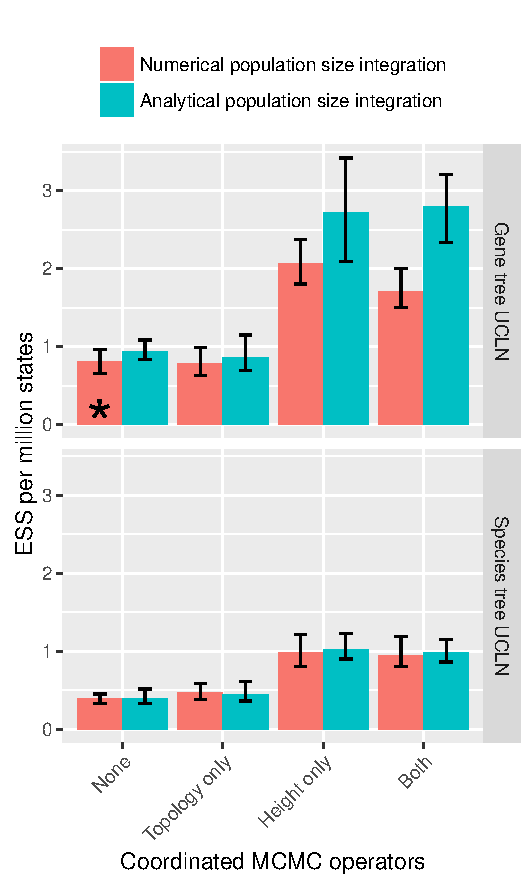
\includegraphics[width=8cm]{speciesTreeHeight_ess_per_mstates.pdf}
\caption
{Effect of operators, population size integration and clock models on effective
sample size (ESS) per million states. The performance of every combination of
settings was measured when applied to 22 \textit{Pseudacris} loci. The bar marked with $\ast$ represents *BEAST
settings, and settings for bars marked with $\ast\ast$ are StarBEAST2 defaults. Topology refers to the
replacement of na\"ive nearest-neighbor interchange and subtree prune and regraft operators with coordinated operators. Height
refers to the addition of operators which make coordinated changes to
node heights. Uncorrelated log-normal (UCLN) relaxed clocks were applied
to either each gene tree or to the species tree. Trimmed means
of species tree height ESS per million states were calculated from
independent chains (N = 32). 25\% trim was used to reduce the influence
of outliers. All error bars are 95\% confidence intervals calculated by
bootstrapping.}
\label{fig:realEssPerMstates}
\end{figure}

\begin{table*}[htb!]
\caption{Change in convergence performance induced by new features}
\label{tab:convergenceLM}
\begin{threeparttable}
\begin{tabular*}{\textwidth}{@{\extracolsep{\fill}}rlrrr@{}}
\hline
Relaxed clock & ESS rate per & Topology & Height & Analytical integration\tabularnewline
\hline
Gene trees & hour & -22\%{***} & 134\%{***} & 23\%{***}\tabularnewline
Gene trees & million states & -5\%\hphantom{***} & 158\%{***} & 26\%{***}\tabularnewline
Species tree & hour & -9\%\hphantom{***} & 114\%{***} & 7\%\hphantom{***}\tabularnewline
Species tree & million states & 6\%\hphantom{***} & 128\%{***} & 9\%\hphantom{***}\tabularnewline
\hline
\end{tabular*}
\begin{tablenotes}
\item {*}: $p < 0.05$, {**}: $p < 0.01$, {***}: $p < 0.001$.
\end{tablenotes}
\end{threeparttable}
\end{table*}

Coordinated height changing operators significantly improved convergence both in
terms of ESS per hour and ESS per million states. Both species and gene
tree relaxed clock analyses benefited from enabling those operators
(Table~\ref{tab:convergenceLM}). Analytical integration of population sizes only
improved the computational performance of gene tree relaxed clock analyses;
unlike height changing operators it did not significantly change the performance
of species tree relaxed clock analyses (Table~\ref{tab:convergenceLM}).

Convergence of species tree relaxed clock analyses was slower than convergence
of gene tree relaxed clock analyses (Figure~\ref{fig:realEssPerHour}). The
decrease in performance was less severe but still present in terms of ESS per
million states (Figure~\ref{fig:realEssPerMstates}), which shows that compared
to gene tree relaxed clock analyses the likelihood calculations have a higher
time cost, but also that operators become less effective at exploring tree and
parameter space.

\subsection{StarBEAST2 is approximately three times faster than *BEAST}

Our reanalysis of \textit{Pseudacris} sequence data shows that analytical
integration of population sizes and coordinated height changing operators both
improve convergence. To show that this increased performance is generally
applicable, and to demonstrate that StarBEAST2 can accurately reconstruct branch
rates under a species tree relaxed clock model, we needed to apply StarBEAST2 to
many different data sets for which the true species tree is known. To accomplish
this we simulated 96 species trees of 19 taxa each under a birth-death model
with log-normally distributed branch rates. Gene trees evolving within each
species tree were simulated according to the MSC model with
log-normally distributed mean clock rates. Finally, sequences were simulated
according to an HKY process for each gene \citep{Hasegawa1985, Goldman1993}. The
parameters used for these simulations were chosen to produce intermediate
branch lengths in coalescent units; the average simulated branch length was
$\nicefrac{1.44\tau}{2Ne}$.

Simulated data was analyzed using concatenation with BEAST and using the MSC with
StarBEAST2. The different settings used for StarBEAST2 were *BEAST settings,
high performance settings with gene tree relaxed clocks, and high performance settings with
species tree relaxed clocks. *BEAST settings matched the configuration of *BEAST
before StarBEAST2; explicit MCMC integration of population sizes, no
coordinated operators, na\"ive NNI and SPR topology operators, and a UCLN
relaxed clock applied to each gene tree. High performance settings included analytical
integration of population sizes, coordinated height changing operators, and
na\"ive NNI and SPR topology operators.

Again the parameter with the slowest convergence given any StarBEAST2 setting
was the height of the species tree (Table~S3,S4). Based on that parameter, the
average performance increase using StarBEAST2 with high performance settings over
*BEAST settings was 3.1 times, with a 95\% confidence interval between 2.7 and
3.6 (Figure~\ref{fig:simulatedEssPerHour}). The slowest converging parameter for
concatenated analyses was the phylogenetic likelihood, and when using the same
number of loci as StarBEAST2, convergence of that statistic using concatenation
was 112 times faster than the convergence of species tree height using
*BEAST settings. When concatenation was used with ten times the
number of loci as StarBEAST2, the performance difference was minimal --- 1.2
times, with a confidence interval between 1.1 and 1.4
(Figure~\ref{fig:simulatedEssPerHour}).

Consistent with analyses of \textit{Pseudacris} sequence data, using a species
tree relaxed clock with high performance settings was faster than *BEAST settings.
Also like \textit{Pseudacris}, use of species tree relaxed clocks was slower than
gene tree relaxed clocks with high performance settings; the average performance
increase over *BEAST settings was only 1.4 times with a confidence interval
between 1.2 and 1.7 (Figure~\ref{fig:simulatedEssPerHour}).

\begin{figure}[htb!]
\centering
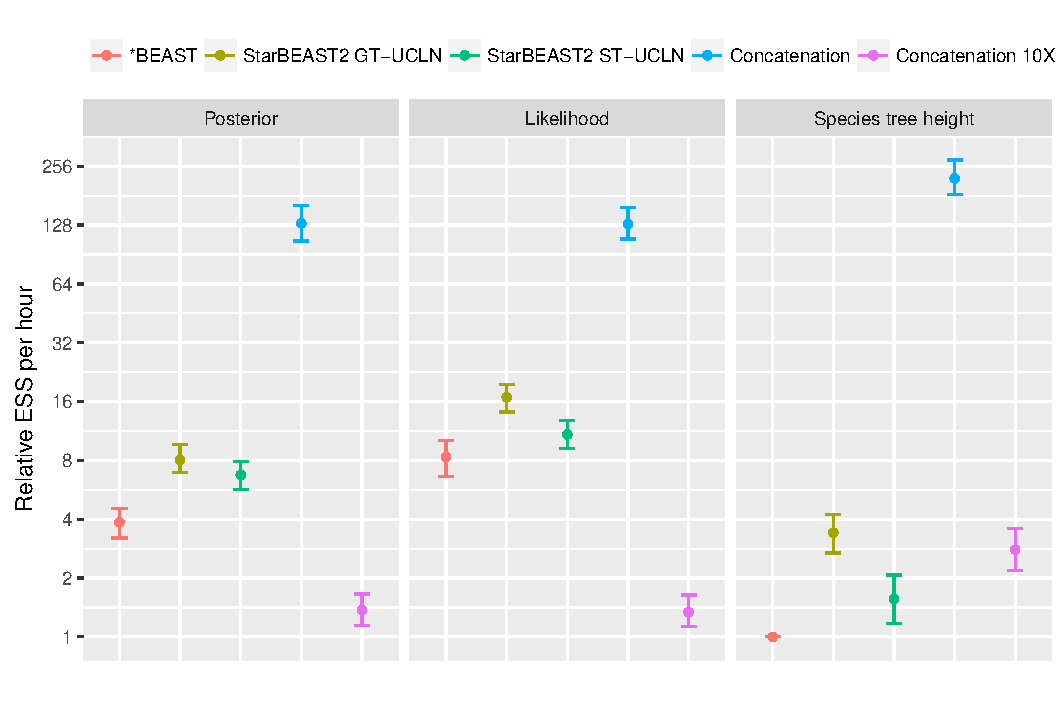
\includegraphics[width=8cm]{multiple_ess_per_hour.pdf}
\caption
{Convergence of different methods applied to simulated data. Methods are
concatenation with 22 loci, concatenation with 220 loci (10X), StarBEAST2 with
*BEAST settings and 22 loci, and StarBEAST2 with high performance settings, 22 loci,
and uncorrelated log-normal relaxed clocks applied to the gene trees (GT-UCLN) or
to the species tree (ST-UCLN). Relative estimated sample size (ESS) per hour is the trimmed mean for all replicates of
ESS per hour divided by species tree height ESS per hour estimated using *BEAST
settings. 25\% trim was used to reduce the influence of
outliers. All error bars are 95\% confidence intervals calculated by
bootstrapping. N = 96.}
\label{fig:simulatedEssPerHour}
\end{figure}

\subsection{Relative accuracy varies according to the type of error}

The accuracy of StarBEAST2 relative to concatenation varied depending on the
type of error and whether equal numbers of loci were used. Relative species tree
error measures the accuracy of estimated branch lengths; by that measure
StarBEAST2 using 22 loci outperformed concatenation using 22 loci, and matched
the performance of concatenation using 220 loci
(Figure~\ref{fig:speciesTreeError}A). Pendant edge bias measures systematic bias
in the estimated ages of extant species; by that measure StarBEAST2 was much
less biased than concatenation regardless of the number of loci
(Figure~\ref{fig:speciesTreeError}B). Rooted Robinson-Foulds distance measures
the topological accuracy of estimated trees; for that metric concatenation using
22 loci was almost as accurate as StarBEAST2, and much more accurate when using
220 loci (Figure~\ref{fig:speciesTreeError}C). For no type of error did the
choice of gene or species tree relaxed clocks affect the accuracy of StarBEAST2
(Figure~\ref{fig:speciesTreeError}A,B,C).

\begin{figure}[htb!]
\centering
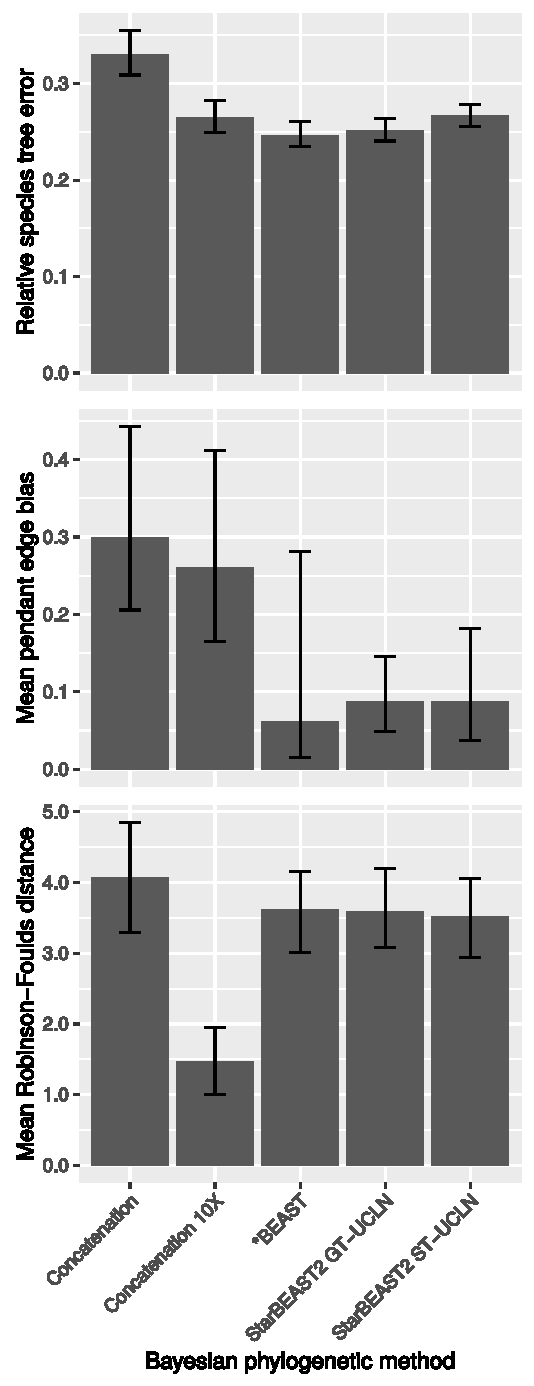
\includegraphics[width=7cm]{tree_error.pdf}
\caption
{Accuracy of different methods applied to simulated data. Methods are concatenation with 22 loci, concatenation with 220 loci
(10X), StarBEAST2 with *BEAST settings and 22 loci, and StarBEAST2 with
high performance settings, 22 loci, and uncorrelated log-normal relaxed clocks applied
to the gene tree (GT-UCLN) or to the species tree (ST-UCLN). (A) Trimmed mean of
relative species tree error, a measure of branch length error. (B) Trimmed
mean of mean pendant edge bias, which measures biased estimates of the ages of
extant species. (C) Trimmed mean of mean rooted Robinson-Foulds distances, a
measure of topological error. 25\% trim was used to reduce the
influence of outliers. All error bars are 95\% confidence intervals calculated
by bootstrapping. N = 96.}
\label{fig:speciesTreeError}
\end{figure}

\clearpage

\subsection{Concatenation cannot accurately infer branch rates given intermediate branch lengths}

While the convergence of species tree relaxed clock analyses was slower than
gene tree relaxed clock analyses using high performance settings, species tree relaxed
clocks enable inference of species branch rates under the MSC. To gauge the
accuracy of estimated branch rates, we used simple linear regressions with the
true rate of each simulated branch as the response variable, and the posterior
expectation of the rate of that branch (conditional on the corresponding clade
being monophyletic in the posterior samples) as the explanatory variable. If all
estimates equal the truth, then the $R^2$ coefficient of determination will
equal 1.

Using either 22 or 220 loci, concatenation was unable to accurately estimate
branch lengths. $R^2$ was very weak at $0.04$ or $0.06$ respectively, and the
deviation from the truth was actually worse when the number of loci was
increased 10-fold (Figure~\ref{fig:deviation}). By applying a relaxed clock to
the species tree, StarBEAST2 can be used to infer many branch rates. Deviation
from the true simulated rates was superior to concatenation
(Figure~\ref{fig:deviation}), and $R^2$ was concordantly higher at $0.17$.

\begin{figure}[htb!]
\centering
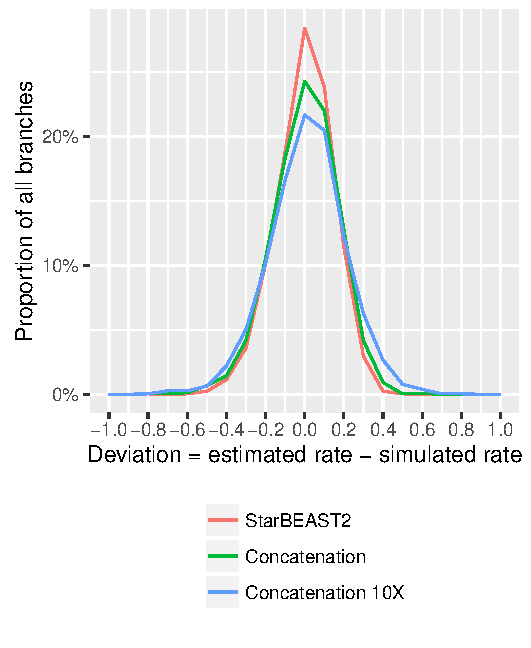
\includegraphics[width=7cm]{branch_rate_deviation.pdf}
\caption
{Deviation of species tree branch rates using concatenation versus StarBEAST2.
Methods are concatenation with 22 loci, concatenation with 220 loci (10X), and
StarBEAST2 with high performance settings, 22 loci, and a relaxed clock applied
to the species tree. Estimated rates are the posterior expectations of each
branch rate from each replicate. Root branch rates, which were fixed at 1.0,
were excluded. N = 96.}
\label{fig:deviation}
\end{figure}

\section{Discussion}

\subsection{StarBEAST2 will enable faster and/or more precise inference}

The increased performance of StarBEAST2 will enable researchers to analyze
results faster and disseminate their findings sooner. A large MCMC analysis
which would currently take three weeks can now be performed in just one week. In
the case of phylogenomic data which has been subsetted for use with *BEAST,
StarBEAST2 can alternatively be used to analyze more data for more precise
estimates of species trees and other parameters in the same amount of time as a
more limited *BEAST analysis.

Previous research on the scaling behaviour of *BEAST has shown that the
relationship between the number of loci in a given analysis and the convergence
in terms of ESS per hour follows a power law with the coefficient $-2.81$ for
the log number of loci \citep{Ogilvie01052016}. If the number of loci for a
given analysis is increased by 50\%, the decrease in performance is therefore
expected to be $\exp(-2.81 \cdot \ln(1.5)) = 3.125$, approximately cancelling
out the improved computational performance of StarBEAST2 compared to *BEAST.

\subsection{Concatenation can still be inferior given intermediate branch lengths}

For short branch lengths in coalescent units, concatenation cannot accurately
estimate branch lengths. *BEAST using just four loci will be more accurate than
concatenation using 4096 loci in terms in relative species tree error and
pendant edge bias. *BEAST will also be more accurate at estimating species tree
topologies given the same number of loci as concatenation, but inferior when
concatenation can be used with a much greater number of loci
\citep{Ogilvie01052016}.

We have shown that concatenation can still be inferior to *BEAST and StarBEAST2
given longer, intermediate branch lengths. For the same number of loci, a higher
relative species tree error indicates that concatenation is less accurate at
estimating branch lengths, and a large pendant edge bias indicates a positive
bias when estimating the ages of extant species. Unlike for short branch
lengths, concatenation with 10 times more loci can catch up to StarBEAST2 in
terms of relative species tree error, but is then slower than StarBEAST2 with
high performance settings. In other words, for intermediate branch lengths StarBEAST2
can be just as accurate as concatenation but needs less investment in both
sequencing and computational time.

Concatenation cannot catch up to StarBEAST2 in terms of pendant edge bias.
Pendant edge bias is important because many published phylogenies show evidence
of a slowdown in diversification rate \citep{Moen2014190}. If the ages of extant
species are overestimated, this will artificially reduce the number of recent
speciation events, mimicking a slowdown. We suggest that accurate inference of
changing diversification rates requires the use of fully Bayesian MSC methods
like StarBEAST2.

\subsection{A multispecies coalescent model is required when inferring species branch rates}

We show that given intermediate branch lengths, concatenation is unable to
accurately estimate per-species substitution rates, and it is reasonable to
assume that shorter branch lengths in coalescent units would exacerbate the
problem. StarBEAST2 can recover many branch rates, and given a more informative
data set than our simulation study of 22$\times$400nt loci should be able to
further improve the accuracy of estimated rates to a point. There are intrinsic
limits to our ability to estimate substitution rates, primarily that branch
length is confounded with substitution rate \citep{Thorne01092002}.

Concatenation is already known to have difficulty inferring substitution rates
because of substitutions produced by ILS (SPILS). When a gene tree contains a
branch absent from the species tree, substitution along that branch must be
attributed to multiple species tree branches in a concatenation analysis,
increasing the substitution rate of those branches. Conversely, when a species
tree contains a branch absent from a gene tree, no substitutions will be
attributed to that branch, decreasing the substitution rate
\citep{Mendes28022016}. This could account for the troubling decline in accuracy
of concatenation when the number of loci is increased.

\section{Conclusions}

When estimating dates and rates, the choice is often between using a subset of
available loci with a fully Bayesian MSC method, or all available loci with
concatenation. Researchers have often opted for the second choice, but we have
shown that concatenation cannot accurately estimate the ages of extant species
or per-species substitution rates, even for trees of intermediate branch lengths. The
increased performance of StarBEAST2 should further encourage the adoption of
fully Bayesian MSC methods for estimating divergence times, and the new species
tree relaxed clock will enable accurate inference of species branch rates despite
ILS. StarBEAST2 is free and open source software, and its source code and
development history is available through GitHub
(\url{https://github.com/genomescale/starbeast2}).

\section{Materials and Methods}

For all StarBEAST2 and concatenation analyses, the version of BEAST used was
2.4.0. For all simulations, the version of biopy used was 0.1.9 (\url{http://www.cs.auckland.ac.nz/~yhel002/biopy/}).

\subsection{Mathematical correctness of StarBEAST2}

Simulated trees were generated using biopy, and trees sampled from a prior
distribution were generated using StarBEAST2 with all new features enabled. This
included analytical integration of population sizes, coordinated tree topology
and node height changing operators, and a species tree relaxed clock. 100,000
species trees were simulated, and 100,000 trees were sampled from the prior at a
rate of one every 1000 after a 10\% burn-in period. Identical parameters were
used for the simulation and for the StarBEAST2 run including the prior
distributions (Table~\ref{tab:correctParameters}). This entire procedure was
repeated separately for UCLN and for UCED species branch rates.

\begin{table}[htb!]
\centering
\caption{Parameters used for verifying correctness}
\label{tab:correctParameters}
\begin{threeparttable}
\begin{adjustbox}{center}
\small
\begin{tabular}{rl}
\hline
Parameter & Distribution\tabularnewline
\hline
Number of species & Fixed at 5\tabularnewline
Birth rate & Fixed at 200.0\tabularnewline
Death rate & Fixed at 100.0\tabularnewline
UCLN branch rates & Log-normal ($\mu^a = 1.0, \sigma = 0.16$)\tabularnewline
UCED branch rates & Exponential ($\lambda = 1.0$)\tabularnewline
Haploid population sizes & Inv. gamma ($\alpha = 2.0, \beta = 0.002$)\tabularnewline
Haplotypes per species & Fixed at 1\tabularnewline
Number of gene trees & Fixed at 2\tabularnewline
Per-locus clock rates & Fixed at 0.5 and 2.0\tabularnewline
\hline
\end{tabular}
\end{adjustbox}
\begin{tablenotes}
\item ${}^a\text{mean in real space}$
\end{tablenotes}
\end{threeparttable}
\end{table}

\subsection{Preprocessing of \textit{Pseudacris} sequence data}

Phased and aligned \textit{Pseudacris} sequence data was retrieved from Dryad
(\url{http://dx.doi.org/10.5061/dryad.23rc0}). In the original analysis, an HKY nucleotide substitution
model was applied to 22 out of 26 nuclear loci \citep{Barrow201478}. To simplify
our reanalysis, which was focused on performance and not reconstructing the
species tree \textit{per se}, we used only those 22 loci. To rank
individual sampled frogs by sequence quality, we counted the number of unambiguous base
calls for both haplotypes across all 22 HKY loci. To further avoid wasting
computational resources, we then reduced the sequence data to both haplotypes
from the best-sequenced individual from each of the 19 extant ingroup lineages
in \cite{Barrow201478}.

\subsection{StarBEAST2 reanalysis of \textit{Pseudacris} sequence data}

For inference of \textit{Pseudacris} trees, we ran 32 independent StarBEAST2
chains for all 16 conditions for a total of 512 chains. The conditions were each
possible combination of species or gene tree relaxed clocks, analytical or
MCMC population size integration, coordinated or na\"ive topology changing
operators, and the inclusion or exclusion of coordinated height changing
operators. Each chain used the same sequence data, but was an independent
estimate of convergence because different random seeds were used to initialize
each chain.

A birth-death prior was used for the species tree and both the net diversification
and extinction fraction hyperparameters were estimated. An inverse gamma prior was
used for per-branch constant population sizes with a shape fixed at 2.0 and the
mean population size hyperparameter was estimated. Relative per-locus clock
rates were estimated using a log-normal prior distribution with the mean fixed
at 1.0 in real space and the standard deviation hyperparameter was estimated. An
HKY+$\Gamma$ substitution model with four gamma rate categories was applied to
all loci and all base frequencies were estimated separately for each locus. The
HKY transition/transversion bias $\kappa$ and gamma shape parameters were estimated and shared across all loci.

The rate of the root species tree branch was estimated for species tree relaxed
clock analyses, but the rates of gene tree root branches were not estimated as
they do not affect the phylogenetic likelihood. The standard deviation of the
UCLN clock model was fixed at 0.16 and 0.32 for species tree and gene tree
relaxed clocks respectively. The number of UCLN rate categories was set to equal
the number of species branches for species tree relaxed clocks (i.e. 37), or
equal the number of gene tree branches excluding the root for gene tree
relaxed clocks (i.e. 74).

To ensure convergence of all chains, we ran each chain for an initial length of
$2^{23}$ states, sampling every $2^{10}$ states. ESS values were computed for
all logged statistics after discarding 12.5\% of state samples as burn-in. Logged
statistics included the posterior probability, the
coalescent probabilities of gene trees, the birth death prior
probability of the species tree, the phylogenetic likelihood, the net
diversification rate, the extinction fraction, the HKY $\kappa$ parameter, the
among-site rate variation $\alpha$ parameter, the standard deviation of
per-locus clock rates, the mean population size, and the height of the species tree.

If any logged statistic had an ESS of below 200, the chain was resumed until the
length of the chain was doubled. ESS values were then re-evaluated, again after
discarding 12.5\% of state samples. The length of the chain was continually
doubled and ESS values re-evaluated until the ESS values of all logged
statistics were above 200. The rate at which trees and statistics were sampled
was halved with every chain doubling so that the total number of samples
remained constant. By the time of submission all chains had converged.

ESS per hour was calculated by dividing the final ESS value for a given
statistic by 87.5\% of the total CPU time used by that chain to account for
burn-in. Likewise ESS per million states was calculated by dividing the final ESS
value by 87.5\% of the total number of the states in the chain. 

Average branch length in coalescent units was calculated by concatenating the
output of the two longest chains using the combination of MCMC population
size integration, na\"ive topology operators, coordinated node height operators
and species tree branch rates. Both chains had been run for $2^{30}$ states for
a total of $2^{31}$ states. For every sample in the combined posterior
distribution, the coalescent length of each branch $\nicefrac{\tau}{2Ne}$ was calculated from the
length in substitution units $\tau$ and effective population size $Ne$ recorded at that
step. The mean coalescent length of all branches across all samples was taken as
the average.

\subsection{Simulation of trees and sequence data}

All simulation parameters were chosen to be broadly similar to those observed in
or estimated from the \textit{Pseudacris} data set.

First, 96 species trees were simulated according to a birth-death process
\citep{Gernhard2008769} using biopy with 19 extant species, a speciation rate of
200.0 and a death rate of 50.0. This corresponds to a net diversification rate
of 150.0 and an extinction fraction of 0.25. Haploid effective population sizes
for each branch were chosen independently from an inverse gamma distribution
with a shape of 2.0 and a scale of 0.002. For a species with annual generation
times, as is the case for at least some \textit{Pseudacris} species
\citep{10.2307/1446044}, this corresponds to a diploid effective population size
of 1000 individuals per generation. Species branch rates were chosen from a
log-normal distribution with a mean in real space of 1.0 and a standard
deviation of 0.16, then scaled so that the mean of the branch rates for a given
species tree was exactly 1.0.

For each species tree, 220 gene trees with two sampled haplotype sequences per species
were simulated according to the MSC process using biopy. The
mean clock rate for each locus was chosen from a log-normal distribution with a
mean in real space of 1.0 and a standard deviation of 0.3. The clock rates of
each sequential block of 22 loci were then scaled so that the mean of the clock
rates for a given block was exactly 1.0. Scaling branch rates and clock rates
was done to ensure that the measured accuracy of StarBEAST2 and concatenation reflected
relative rather than absolute differences between simulated and estimated times
and rates.

For each gene tree, 400nt long sequence alignments were simulated using Seq-Gen
\citep{Rambaut01061997}. An HKY model was used for all sequence alignments with
equal base frequencies, a $\kappa$ value of 3.0, and a four rate category discretized gamma model
of among-site rate variation with a shape $\alpha$ value of 0.2
\citep{Yang1994}.

\subsection{Performance and accuracy of StarBEAST2 and concatenation}

The five methods of inference used for this section were concatenation with 22
loci, concatenation with 220 loci, StarBEAST2 with *BEAST settings, StarBEAST2
with high performance settings and gene tree relaxed clocks, and StarBEAST2 with
high performance settings and species tree relaxed clocks. A single MCMC chain was
run for each method of inference for all 96 replicates, a total of 480 chains.

The settings used for StarBEAST2 analyses of simulated sequence data were
identical to the analysis of \textit{Pseudacris} sequence data, except that 100
rate categories were used for all UCLN relaxed clocks. Concatenation used the
same settings as StarBEAST2, but instead of inferring each gene tree within a
species tree, a single concatenated tree was inferred using the likelihoods of
all loci. In addition to the rates of concatenated tree branches, we estimated
the per-gene rates, a model equivalent to that described by \cite{Rasmussen01122007}.
Heterozygous sites were ambiguity coded for concatenation analyses.

The same strategy to ensure convergence was used as for \textit{Pseudacris}
analyses, but slightly modified for concatenated analyses; mean population sizes
and coalescent probabilities were not logged because they are not estimated, and
the initial chain length was only $2^{20}$ states, sampling every $2^{7}$
states. By the time of submission all chains had converged. ESS per hour and ESS
per million states were calculated using all chains regardless of convergence in
the same way as for \textit{Pseudacris}. Measures of accuracy were calculated
from only the converged chains.

Relative species tree error is based on ``rooted branch score''
\citep[RBS;][]{Heled2013}. Given two trees $T_1$ and $T_2$, the sets of
monophyletic clades $c$ present in each tree are defined as $\mathbb{C}_1$ and
$\mathbb{C}_2$. The length of the parent branch extending from the root of the
subtree defined by $c$ is then $b(c)$. To calculate the rooted branch score, sum
all absolute differences in $b(c)$ between trees $T_1$ and $T_2$:

\begin{equation}
RBS(T_1, T_2) = \sum_{c \in {\mathbb{C}_1} \cup {\mathbb{C}_2}} |b^{(1)}(c) - b^{(2)}(c)|
\end{equation}

If a clade $c$ is present in only one of $T_1$ or $T_2$, then the branch length
$b(c)$ from the tree containing $c$ is added to the RBS. Relative species tree
error is the mean RBS between an estimated species tree and the true
species tree over the posterior distribution of species trees, and is normalized
by dividing by the total length of the true species tree
\citep{Ogilvie01052016}.

Pendant edge bias is defined as $\nicefrac{\hat{h} - h}{h}$, where the estimated
age for each extant species is $\hat{h}$ and the true age is $h$. The mean
pendant edge bias is the average pendant edge bias for all extant species across
all posterior samples.

Rooted Robinson-Foulds distances \citep{ROBINSON1981131} are defined as the
count of clades present only one of $T_1$ and $T_2$. In this study, the mean
rooted Robinson-Foulds distance is the average of all distances between each
estimated tree and the true tree for all posterior samples.

\section{Supplementary Material}
Supplementary tables S1--S4 and figures S1--S6 are available at Molecular Biology and Evolution
online (http://www.mbe.oxfordjournals.org/).

\section{Acknowledgments}

This work was supported by a Rutherford Discovery Fellowship awarded to A.J.D. by
the Royal Society of New Zealand. H.A.O. was supported by an Australian Laureate
Fellowship awarded to Craig Moritz by the Australian Research Council
(FL110100104). This research was undertaken with the assistance of resources
from the National Computational Infrastructure (NCI), which is supported by the
Australian Government. We wish to thank Jason Bragg and Renee Catullo for
testing StarBEAST2 before its official release, Tim Vaughan for suggesting the
addition of the root height changing operator, Joseph Heled for insight into the
multispecies coalescent, and Graham Jones for input regarding operator
performance.

\bibliographystyle{natbib}%%%%natbib.sty
\bibliography{starbeast2-mbe}%%%refs.bib

\end{document}
